\begin{frame}
  \frametitle{Assumptions}

  \begin{itemize}
  
  \item New Nuclear = Advanced Boiling Water Reactors \cite{rothwell_real_2006}.
  
  \item Simplistic, conservative assumption about demand growth = +1.7\% per year\cite{noauthor_electricity_2017}.
  
  \item Nuclear, wind, solar annual growth rate \textbf{limits} based on trends in USA, China, Japan \cite{noauthor_electricity_2017,noauthor_energy_2018,eia_international_nodate,eia_monthly_2018,iea-pvps_snapshot_2018}.
  
  \item CCS: Available for deployment in 2030, costs reduce by 2050 \cite{kato_energy_2016}.
  
  \item Offshore and onshore wind capacity limited to theoretical potential (about 450 GW and 200 GW respectively).
  
  \item H$_2$: Steam reforming available in 2030, photocatalytic conversion in 2050 (assumed cost-competitive with other generation methods) \cite{kato_energy_2016} \cite{acar_comparative_2014}.
  
  \item Hydropower, geothermal capacity held constant \cite{noauthor_energy_2018}.
  
  \end{itemize}

\end{frame}


\begin{frame}
  \frametitle{Levelized cost projections for solar and wind}
  \begin{figure}[htbp!]
    \begin{center}
      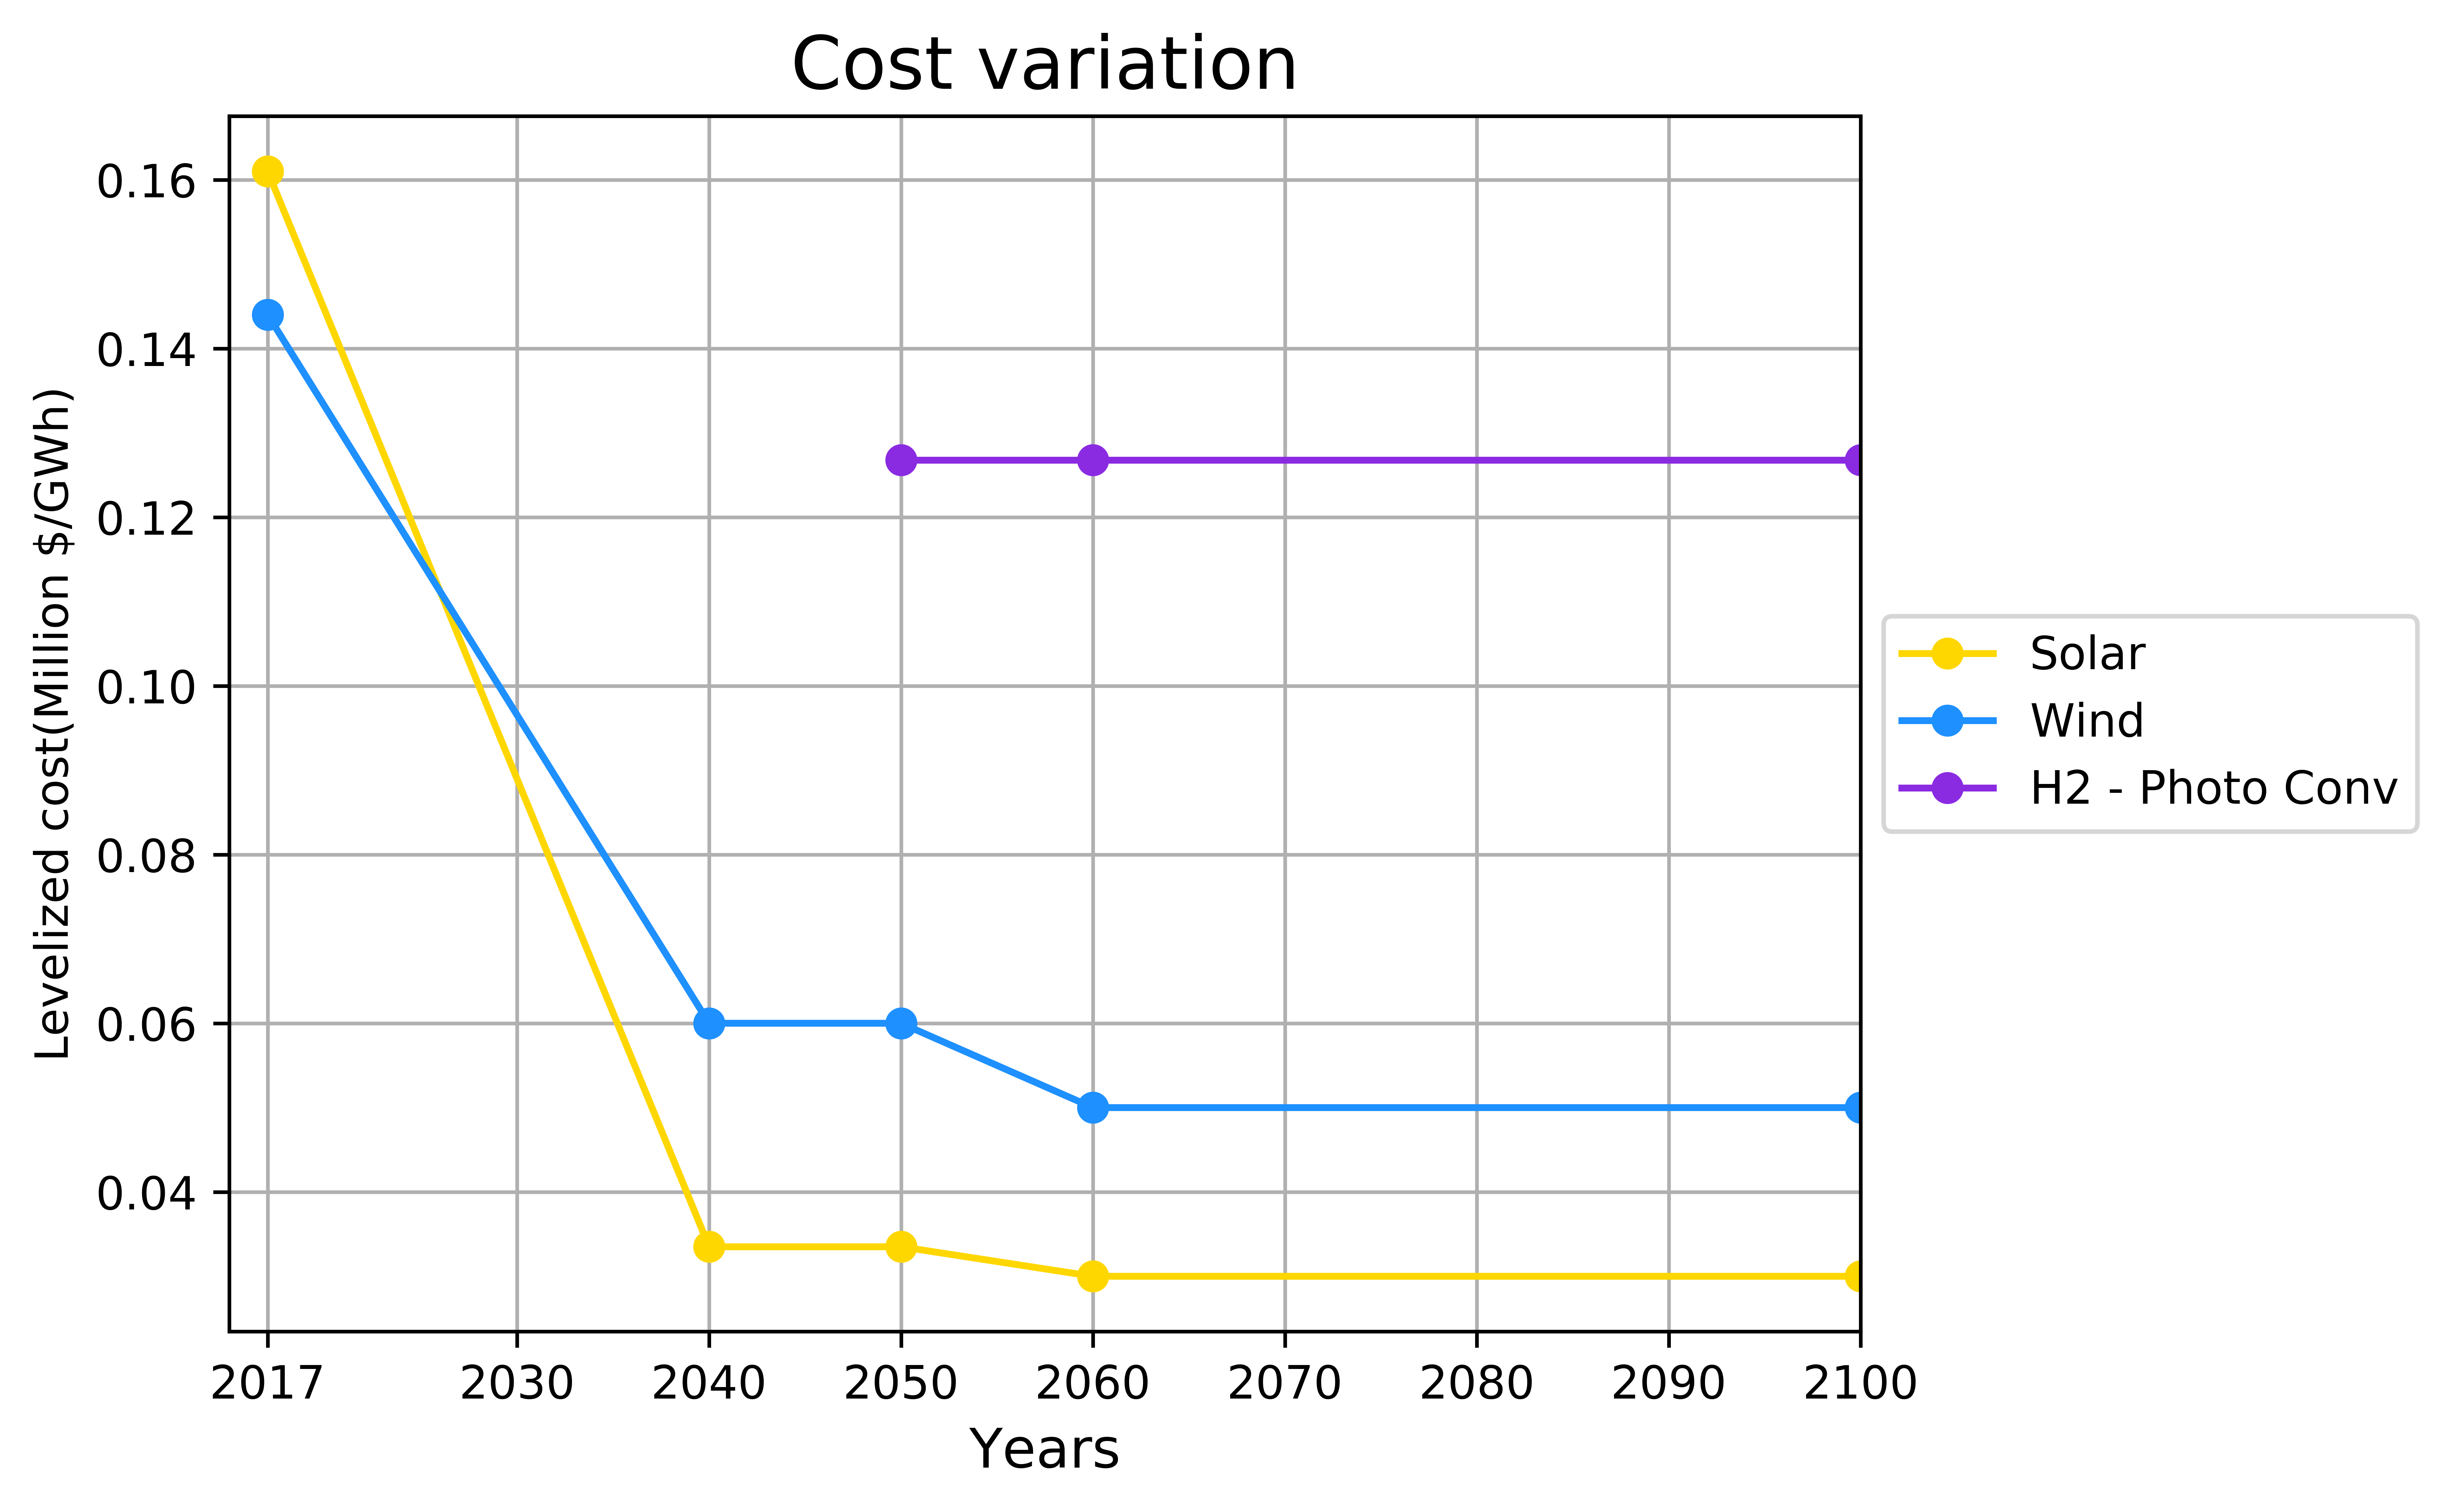
\includegraphics[scale=0.5]{./images/cost}
    \end{center}
          \caption{Levelized cost projections from Lazard \cite{noauthor_lazards_2017} and Acar \& Dincer \cite{acar_comparative_2014}}
    \label{cost}
  \end{figure}
\end{frame}

\begin{frame}
\frametitle{Contribution to peak factor (C2P factor)}
This is a TIMES parameter that defines what fraction of a energy source's capacity is guaranteed to be available during peak demand \cite{loulou_etsap-tiam:_2008}.\\

\begin{tabular}{|c|c|}
\hline 
\textbf{Energy source} & \textbf{C2P factor} \\
\hline 
Fossil fuels & 1 \\
Nuclear power & 1 \\
Solar power & 0.42 \cite{kato_energy_2016}\\
Wind & 0.20 \cite{nguyen_factors_2016}\\
\hline 
\end{tabular}

This factor is reduced for solar and wind with increasing penetration \cite{nguyen_factors_2016}.
\end{frame}